% =====================================================================
%  Parcial práctico de Ingeniería de Software: La última transmisión
%  Informe y anexos en un solo documento. Compilar con pdfLaTeX.
% =====================================================================
\documentclass[11pt,letterpaper]{article}

% ---------- Idioma y tipografía ----------
\usepackage[utf8]{inputenc}
\usepackage[T1]{fontenc}
\usepackage[spanish,es-noshorthands,es-tabla,es-nodecimaldot]{babel}
\usepackage{newtxtext,newtxmath}      % Times
\usepackage[scaled=0.88]{beramono}    % monoespaciada para código y rutas
\usepackage{microtype}

% ---------- Página ----------
\usepackage[letterpaper,top=2.2cm,bottom=2.2cm,left=2.5cm,right=2.5cm]{geometry}
\usepackage{setspace}
\setstretch{1.0}
\setlength{\parindent}{0pt}
\setlength{\parskip}{3pt}

% ---------- Paquetes ----------
\usepackage{xcolor}
\usepackage{graphicx}
\usepackage{booktabs,tabularx,longtable,array}
\usepackage{enumitem}
\usepackage{float}
\usepackage{caption}
\usepackage{titlesec}
\usepackage{tikz}
\usetikzlibrary{arrows.meta,positioning,shapes.geometric,shapes.multipart,fit,calc,backgrounds}
\usepackage{pgf-umlcd}
\usepackage{pgf-umlsd}
\usepackage{xurl}
\usepackage[hidelinks]{hyperref}
\urlstyle{tt}

% ---------- Estilo ----------
\titleformat{\section}{\normalfont\large\bfseries}{\thesection.}{0.5em}{}
\titleformat{\subsection}{\normalfont\normalsize\bfseries}{\thesubsection.}{0.5em}{}
\titlespacing*{\section}{0pt}{12pt}{4pt}
\titlespacing*{\subsection}{0pt}{8pt}{2pt}
\setlist{itemsep=1pt,topsep=2pt,leftmargin=1.4em}
\captionsetup{font=small,labelsep=period}
\renewcommand{\arraystretch}{1.2}
\newcolumntype{L}{>{\raggedright\arraybackslash}X}
\renewcommand{\umldrawcolor}{black}
\renewcommand{\umlfillcolor}{white}
\tikzset{drop shadow/.style={}}

\newcommand{\cod}[1]{\texttt{#1}}
% Marca lo que falta por completar. Bórrenla cuando terminen.
\newcommand{\pendiente}[1]{\textcolor{red}{[COMPLETAR: #1]}}

% ---------- Datos de la entrega (EDITAR) ----------
\newcommand{\integranteA}{Juan Manuel Rudas Tijera}
\newcommand{\codigo}{T00067552}
\newcommand{\integranteB}{Luis Carlos Corredor Altamiranda}
\newcommand{\codigoB}{T00083513}
\newcommand{\docente}{Aisner Marrugo}
\newcommand{\repo}{https://github.com/JuanRudas02/trabajo-ingenieria-software}

\begin{document}

% =====================================================================
%  IDENTIFICACIÓN
% =====================================================================
\begin{center}
{\large Universidad Tecnológica de Bolívar}\\
Ingeniería de Software\\[10pt]
{\Large\bfseries Motor de historias interactivas}\\[2pt]
{\large Parcial práctico: \textit{La última transmisión}}\\[10pt]
\integranteA\ (\codigo)\\
\integranteB\ (\codigoB)\\[2pt]
Docente: \docente\\
Repositorio: \url{\repo}\\
Cartagena, \today
\end{center}
\vspace{2pt}
\noindent\rule{\linewidth}{0.4pt}

% =====================================================================
\section{Fundamentos}
% =====================================================================
\subsection{Problema, actores y alcance}
Un colectivo de escritores quiere publicar una historia interactiva para un festival universitario sin depender de un programador cada vez que cambie una escena. Necesitan escribir la historia en un archivo, que las opciones dependan de lo que el lector ya descubrió y que los errores del archivo aparezcan antes de que alguien juegue.

Los actores son la escritora, que crea y corrige los archivos; el lector, que juega; el diseñador de la experiencia, que define condiciones y consecuencias; y la coordinadora del festival, que no acepta cierres inesperados del programa. La Figura~\ref{fig:contexto} muestra el contexto.

El alcance de la primera versión incluye cargar historias en JSON, validarlas antes de jugar, mostrar escenas y opciones condicionadas, aplicar efectos booleanos, detectar finales y bloqueos, y reiniciar. Desde la versión \cod{v1.1} incluye además deshacer la última decisión (sección~\ref{sec:cambio}). Quedan por fuera rehacer, el retroceso de varios niveles, las cuentas de usuario, la base de datos, el guardado entre ejecuciones, la red, el editor visual, los elementos multimedia y cualquier lenguaje de expresiones.

\subsection{Riesgos}
\begin{enumerate}[label=R\arabic*.]
  \item \textit{La solicitud de cambio de la hora 6 obliga a rehacer partes del diseño.} Para mitigarlo el sistema se separó en capas, la versión \cod{v1.0} se etiqueta en Git antes de recibir el cambio y se mantiene una suite de regresión que se corre después de cada modificación.
  \item \textit{Un archivo de historia con errores llega al lector.} Para mitigarlo, el archivo se valida completo antes de crear la partida (nueve categorías de error) y el README trae el formato y una historia de ejemplo para copiar.
\end{enumerate}

\subsection{Atributos de calidad}
El orden de prioridad es el siguiente: primero la confiabilidad, porque la coordinadora exige que el programa no se cierre de forma inesperada; después la modificabilidad del contenido, porque la escritora no programa; luego la claridad de los errores, sin la cual la modificabilidad no sirve; después la facilidad de uso de la consola y, al final, el rendimiento, que no es un problema con historias de pocas decenas de escenas.

\subsection{Responsabilidad profesional}
El motor nunca escribe sobre los archivos de historia: el texto es del colectivo y el programa solo lo lee. No se guardan datos de los lectores. En cuanto a dependencias, el producto usa solo la biblioteca estándar de Python, y \cod{pytest} (licencia MIT) se usa únicamente para las pruebas, así que no se distribuyen bibliotecas de terceros con el juego. El uso de herramientas de IA se declara en la sección~\ref{sec:fuentes}.

% =====================================================================
\section{Proceso}
% =====================================================================
Trabajé con un proceso incremental. Hubo tres incrementos internos: \cod{v0.1} con el contenido y la validación, \cod{v0.2} con las reglas de la sesión y \cod{v1.0} con la consola y la integración. Después se hace \cod{v1.1} con la solicitud de cambio.

Lo comparé con cascada. Cascada supone requisitos estables desde el principio, pero la guía anuncia un cambio a mitad de la ventana. Con un incremento funcional y probado en la hora 6, el cambio se aplica sobre algo que ya funciona; en cascada me encontraría con la implementación a medias.

\begin{tabularx}{\linewidth}{@{}lL@{}}
\toprule
Actividad & Cómo la realicé en esta entrega\\ \midrule
Especificación & RF atómicos con criterio de aceptación (sección~\ref{sec:req}), revisados con una lista de chequeo (atomicidad, verificabilidad y cobertura de N01 a N06) antes de programar.\\
Desarrollo & Por incrementos. Cada criterio de aceptación se escribió primero como prueba en \cod{pytest}.\\
Validación & Suite automatizada de 86 casos, más el recorrido manual de los tres finales y de la segunda historia.\\
Evolución & Etiqueta \cod{v1.0}, análisis de impacto de la solicitud y \cod{v1.1} con la trazabilidad actualizada (sección~\ref{sec:cambio}).\\ \bottomrule
\end{tabularx}

% =====================================================================
\section{Agilidad}
% =====================================================================
Usé un tablero Kanban con las columnas Por hacer, En curso, Revisión y Hecho. El tablero está en GitHub Projects, vinculado al mismo repositorio, y cada elemento del backlog es un \textit{issue}; la captura del tablero está en el Anexo~\ref{anx:tablero}.

\begin{tabularx}{\linewidth}{@{}llLll@{}}
\toprule
ID & Prioridad & Elemento del backlog & Responsable & Estado\\ \midrule
B1 & Alta & Modelo de dominio y cargador JSON (RF01) & J. Rudas & Hecho\\
B2 & Alta & Validador con nueve categorías de error (RF11) & J. Rudas & Hecho\\
B3 & Alta & Sesión: condiciones, efectos y rechazo sin cambios (RF02--RF08) & J. Rudas & Hecho\\
B4 & Alta & Finales, reinicio y bloqueo (RF09, RF10, RF12) & J. Rudas & Hecho\\
B5 & Media & Consola y entradas inválidas (RF03, RF07) & J. Rudas & Hecho\\
B6 & Media & Segunda historia y pruebas de RNF & J. Rudas & Hecho\\
B7 & Media & Requisitos, modelos, arquitectura e informe & J. Rudas & Hecho\\
B8 & Alta & Solicitud de cambio de la hora 6: deshacer (RF13) & J. Rudas & Hecho\\ \bottomrule
\end{tabularx}

\subsection{Prácticas}
Apliqué dos prácticas. La primera fue limitar el trabajo en curso a una sola tarea a la vez en el tablero, para no tener varias piezas a medias cuando llegara el cambio. La segunda fue escribir las pruebas de los criterios de aceptación antes del código: CA01 a CA03 y U1 a U5 se convirtieron en pruebas que fallaban hasta que la funcionalidad estuvo lista. Descarté Scrum con sprints y ceremonias formales, porque en una ventana de 12 horas la planificación, la revisión y la retrospectiva de cada sprint cuestan más de lo que aportan.

\subsection{Definición de terminado}
Una tarea está terminada cuando su código está en la rama principal, todas las pruebas pasan, los requisitos y la matriz de trazabilidad están actualizados, pasó la lista de chequeo de revisión y el README sigue siendo correcto.

\subsection{Aprendizaje}
La primera versión de la prueba de robustez, con 1000 entradas aleatorias, falló porque no simulaba el fin de la entrada estándar y se quedaba esperando una respuesta. Como acción de mejora, todas las pruebas de consola usan ahora una fuente de entrada que termina con \cod{EOFError}, que es el mismo caso que el programa ya trata como una salida controlada.

% =====================================================================
\section{Requerimientos}\label{sec:req}
% =====================================================================
\subsection{Requisitos funcionales}
{\small
\begin{longtable}{@{}>{\raggedright}p{0.95cm}>{\raggedright}p{0.75cm}>{\raggedright}p{5.4cm}>{\raggedright\arraybackslash}p{8.1cm}@{}}
\toprule
ID & Nec. & El sistema debe & Criterio de aceptación\\ \midrule\endhead
RF01 & N01 & Cargar una historia desde la ruta de archivo que se indica al ejecutar el programa. & Al ejecutar \cod{jugar.py} con \cod{historias/el\_faro.json} se muestran el título y la escena F1.\\
RF02 & N01 & Iniciar cada partida en la escena \cod{inicio} con los valores de \cod{variables} del archivo. & Al iniciar, la escena es E1 y las dos variables valen \cod{false}.\\
RF03 & N02 & Mostrar el texto de la escena actual. & Después de elegir ``Revisar señal'' se muestra el texto de E2.\\
RF04 & N02 & Mostrar solo las opciones cuyas condiciones son todas iguales al valor actual de cada variable. & CA01: después de ``revisar'' e ``investigar'', en E3 se muestran exactamente ``Activar con código'' y ``Cortar comunicación''.\\
RF05 & N03 & Aplicar a las variables los efectos de la opción elegida. & Después de ``investigar'', \cod{conoce\_origen} vale \cod{true}.\\
RF06 & N03 & Llevar a la escena destino de la opción elegida. & Después de ``investigar'' la escena actual es E3.\\
RF07 & N03 & Rechazar una opción inexistente, no habilitada o una entrada no numérica sin cambiar la escena ni las variables. & CA02: en E3 sin conocer el origen, \cod{elegir("activar\_codigo")} devuelve \cod{aceptada = false} y el estado queda igual.\\
RF08 & N04 & Conservar el valor de las variables durante toda la partida. & El efecto aplicado en E2 determina las opciones de E3 en la misma partida.\\
RF09 & N05 & Informar el desenlace al llegar a una escena con \cod{final = true}. & Al llegar a E4, E5 o E6 se muestra ``FIN DE LA HISTORIA''.\\
RF10 & N05 & Reiniciar restaurando la escena y las variables iniciales, sin datos de la partida anterior. & Después de terminar en E4 y reiniciar, en E3 sin investigar aparece ``Activar sin verificar''.\\
RF11 & N06 & Validar el archivo antes de crear la partida y, si tiene errores, rechazarlo listando cada uno con su categoría, causa y campo o ID. & CA03: con un destino E99 no se abre la partida y se muestra \cod{[DESTINO\_INEXISTENTE] escena E3.opcion cortar.destino}.\\
RF12 & N06 & Informar un bloqueo cuando una escena no final no tiene opciones habilitadas, y ofrecer reiniciar. & Con una historia cuya E3 solo tiene ``activar\_codigo'', al llegar sin investigar se muestra ``[BLOQUEO]'' y se ofrece reiniciar.\\
RF13 & N03, N04 & Deshacer la última elección válida, restaurando exactamente la escena y las variables previas a ella; un solo nivel, disponible también desde un final y eliminado al reiniciar. & Desde E2, ``investigar'' lleva a E3 con \cod{conoce\_origen = true}; deshacer vuelve a E2 con \cod{false}; un segundo deshacer no cambia nada; al elegir ``continuar'', E3 muestra ``Activar sin verificar'' y ``Cortar comunicación''.\\ \bottomrule
\end{longtable}}

\subsection{Requisitos no funcionales}
{\small
\begin{tabularx}{\linewidth}{@{}>{\raggedright}p{2.3cm}>{\raggedright}p{5.4cm}L@{}}
\toprule
ID y atributo & Requisito & Procedimiento, evidencia y resultado\\ \midrule
RNF01\newline Modificabilidad & Una historia nueva que cumpla el formato se juega hasta un final sin modificar ningún archivo de \cod{motor/}, y el código del motor no contiene IDs ni variables de ninguna historia. & \cod{test\_rnf.py::test\_RNF01} calcula el SHA-256 de \cod{motor/*.py} antes y después de jugar \cod{el\_faro.json} y busca IDs en el código. Además, \cod{git diff --stat -- motor/} en el commit que agrega la historia. Resultado: 0 archivos modificados.\\
RNF02\newline Claridad de errores & El 100\,\% de los errores de contenido (18 variantes de las ocho categorías que se detectan al cargar) produce un mensaje con categoría, causa y campo o ID, sin trazas de pila. & \cod{test\_rnf.py::test\_RNF02}, prueba parametrizada con 18 casos. Resultado: 18 de 18.\\
RNF03\newline Confiabilidad & Ninguna terminación no controlada con 1000 entradas aleatorias en la consola (semilla 2026) y ningún cambio de estado con 1000 elecciones inválidas. & \cod{test\_rnf.py::test\_RNF03}, dos pruebas. Resultado: 0 terminaciones y 0 cambios. Registro en \path{resultados/ultima_ejecucion.txt}.\\ \bottomrule
\end{tabularx}}

\subsection{Preguntas y supuestos}
\begin{enumerate}[label=P\arabic*.]
  \item ¿Son obligatorios \cod{condiciones} y \cod{efectos} aunque estén vacíos? No obtuve respuesta durante la ventana. Supuesto: sí, porque el contrato los lista como campos de la opción; un mapa vacío se escribe \cod{\{\}}. Quedó documentado en el README.
  \item ¿Qué se hace con campos que el contrato no menciona, por ejemplo notas de la escritora? Supuesto: se ignoran, porque no afectan las reglas y le facilitan el trabajo editorial.
  \item ¿Puede repetirse el ID de una opción en escenas distintas? La guía responde que sí: la unicidad es dentro de la escena. Lo verifiqué con una prueba.
\end{enumerate}

\subsection{Conflicto sobre el retroceso}\label{sec:retroceso}
La escritora quiere poder retroceder siempre y el diseñador quiere decisiones irreversibles. La pregunta de aclaración para el cliente es: ``Si se permite retroceder, ¿también deben deshacerse los efectos sobre las variables? ¿Hay escenas que el diseñador quiera marcar como irreversibles?''. Mientras no haya respuesta, el acuerdo provisional es que la primera versión no tiene retroceso: las decisiones son irreversibles y la única forma de volver es reiniciar. No dejé nada implementado a la espera de esa decisión. En la hora 6 el cliente resolvió el conflicto: el lector puede deshacer su última decisión, con todas sus consecuencias. Esa decisión reemplazó el acuerdo provisional y se implementó como RF13 (sección~\ref{sec:cambio}).

\subsection{Revisión cruzada}
Al revisar los requisitos con la lista de chequeo encontré una ambigüedad. La primera redacción de RF04 decía ``mostrar las opciones válidas'', lo que no se podía verificar porque ``válidas'' también podía entenderse como ``bien escritas''. La corregí a ``cuyas condiciones son todas iguales al valor actual''. Esa corrección dejó ver un error frecuente: si se evalúa \cod{if variables[k]} en lugar de comparar igualdad, ``Activar sin verificar'' (que exige \cod{false}) nunca aparece. Agregué la prueba \cod{test\_U1\_condicion\_false\_se\_evalua\_por\_igualdad}.

También encontré un defecto en el cargador: el módulo \cod{json} de Python acepta claves repetidas en un objeto y se queda con la última sin avisar. Lo corregí con un \cod{object\_pairs\_hook} que rechaza las claves repetidas, con su prueba \cod{clave\_repetida}.

% =====================================================================
\section{Modelado}
% =====================================================================
Los diagramas están en el Anexo~\ref{anx:uml} y usan los mismos nombres que el código (\cod{Historia}, \cod{Escena}, \cod{Opcion}, \cod{Sesion}, \cod{condiciones}, \cod{efectos}).
\begin{itemize}
  \item Contexto (Figura~\ref{fig:contexto}): el motor es una aplicación local y su único sistema externo es el archivo de historia.
  \item Casos de uso (Figura~\ref{fig:cu}): CU01 a CU09, relacionados con RF01 a RF13. CU09 (Deshacer última decisión) se agregó con la solicitud de cambio.
  \item Clases (Figura~\ref{fig:clases}): las clases del dominio son inmutables y \cod{Sesion} es la única con estado que cambia. La regla de igualdad está en \cod{Opcion.habilitada()}.
  \item Secuencia (Figura~\ref{fig:secuencia}): elegir una opción. La consola convierte el número en un ID y la sesión vuelve a validar antes de aplicar los efectos.
  \item Estados (Figura~\ref{fig:estados}): Cargando, Rechazada, EnEscena, Bloqueada y Terminada. Las elecciones inválidas son transiciones al mismo estado, sin efectos. La versión \cod{v1.1} agrega la transición \cod{deshacer()} desde EnEscena, Terminada y Bloqueada.
\end{itemize}
El mapa narrativo (Figura~\ref{fig:mapa}) describe los datos de la historia; no reemplaza los modelos del software.

% =====================================================================
\section{Arquitectura}
% =====================================================================
El sistema tiene tres capas y cada una depende solo de la que está debajo (Figura~\ref{fig:componentes}). La interfaz (\cod{jugar.py}) lee el teclado, imprime y maneja el menú de reinicio. Las reglas (\cod{sesion.py}) guardan el estado y evalúan condiciones y efectos. El contenido (\cod{cargador.py}, \cod{validador.py}, \cod{modelo.py} y \cod{errores.py}) lee, valida y representa la historia. Las historias son datos y están en la carpeta \cod{historias/}.

El contenido se separó del motor para que la escritora pueda cambiar la historia sin tocar código (N01, RNF01). Las reglas se separaron de la interfaz para que la sesión no imprima ni lea del teclado; por eso CA02 y U1 a U5 se prueban sin consola, y una interfaz web podría usar la misma clase. La prueba práctica es \cod{el\_faro.json}: cuatro escenas, una condición y un efecto, que se juegan con el mismo motor sin modificarlo.

\subsection{Decisión 1: estilo de arquitectura}
\textit{Contexto.} Se espera un cambio de requisitos a mitad de la ventana y hay que cargar una segunda historia sin editar el motor.
\textit{Alternativas.} Un script único; MVC; capas de contenido, reglas e interfaz.
\textit{Elección.} Capas.
\textit{Consecuencias.} Las reglas se prueban sin entrada ni salida y los cambios de formato quedan aislados en el cargador y el validador. A cambio hay más archivos y una indirección más para un programa pequeño. MVC no se justificaba porque no hay varias vistas.

\subsection{Decisión 2: cuándo y cómo validar}
\textit{Contexto.} El lector no debe encontrarse con errores (N06) y la escritora necesita saber qué corregir.
\textit{Alternativas.} Validar cada escena cuando se visita; validar todo antes de jugar y parar en el primer error; validar todo antes de jugar y reunir todos los errores.
\textit{Elección.} La tercera.
\textit{Consecuencias.} Ningún archivo inválido llega a abrir una partida (CA03) y la escritora corrige todo en una sola pasada. A cambio, el validador tiene que seguir revisando aunque la estructura esté parcialmente rota, lo que exige más comprobaciones de tipo. Los bloqueos que dependen del camino recorrido solo se detectan durante la partida (RF12), algo que la guía permite.

% =====================================================================
\section{Implementación y pruebas}
% =====================================================================
Usé Python 3.10 o superior (probado en 3.13) con interfaz de consola. Las bibliotecas son las de la biblioteca estándar (\cod{json}, \cod{dataclasses}, \cod{pathlib}, licencia PSF) y \cod{pytest} 9.1 (licencia MIT), solo para las pruebas.

\subsection{Decisión de diseño detallado}
\cod{Sesion.elegir(id)} primero busca la opción en la escena actual y verifica que esté habilitada. Solo si las dos comprobaciones pasan crea un diccionario nuevo de variables con los efectos y cambia de escena. Así una entrada inválida nunca deja el estado a medias (U3) y la consola no puede saltarse la regla enviando el ID de una opción oculta (CA02). Las variables se entregan como copia para que nadie pueda modificar el estado desde fuera, y \cod{reiniciar()} crea una copia nueva de las variables iniciales; si se reutilizara el diccionario cargado del archivo, una partida dejaría rastros en la siguiente (N05). La regla de igualdad vive en \cod{Opcion}, que es la clase que tiene la información, y eso reduce el acoplamiento entre \cod{Sesion} y el formato de las condiciones.

\subsection{Pruebas}
{\small
\begin{tabularx}{\linewidth}{@{}l>{\raggedright}p{6.4cm}L@{}}
\toprule
Caso & Entrada y resultado esperado & Prueba y resultado\\ \midrule
U1 & E3 con \cod{conoce\_origen} verdadero o falso: [activar\_codigo, cortar] o [activar\_sin\_verificar, cortar] & \cod{test\_sesion::test\_U1\_*}, 3 casos, pasan\\
U2 & ``investigar'' en E2: pasa a E3 con \cod{conoce\_origen = true} & \cod{test\_sesion::test\_U2\_*} y \cod{test\_CA01}, pasan\\
U3 & Seis entradas inválidas (inexistente, de otra escena, no habilitada, en un final, vacía): estado igual & \cod{test\_sesion::test\_U3\_*}, 6 casos, pasan\\
U4 & 22 archivos con errores: \cod{ErrorContenido} con categoría y ubicación & \cod{test\_validacion::test\_U4\_*}, 22 casos, pasan\\
U5 & Terminar en E4 y reiniciar: E1 con variables iniciales y sin historial de retroceso & \cod{test\_sesion::test\_U5\_*}, 3 casos, pasan\\
U6 & Deshacer: restaura escena y variables, consume el retroceso, no existe al inicio, la entrada inválida preserva el historial y una nueva elección lo habilita & \cod{test\_deshacer::test\_U6\_*}, 12 casos, pasan\\
I1 & Archivo real hasta E4, E5 y E6; deshacer desde cada final; consola con entradas inválidas, deshacer y reinicio & \cod{test\_integracion::test\_I1\_*}, 8 casos, pasan\\ \bottomrule
\end{tabularx}}

Las pruebas de validación cubren las nueve categorías de error: archivo ilegible o con estructura incorrecta, campo obligatorio ausente, inicio inexistente, ID repetido (de escena, o de opción dentro de su escena), destino inexistente, variable no declarada, valor no booleano, cantidad de opciones incompatible con \cod{final}, y bloqueo durante la partida (\cod{test\_bloqueo\_en\_ejecucion\_*}).

\subsection{Verificación del producto}
Los tres finales se alcanzan con las rutas que indica el README, \cod{el\_faro.json} se juega hasta sus dos finales y los tres RNF se cumplen. En la última ejecución (versión \cod{v1.1}) pasaron las 86 pruebas, sin fallos (\path{resultados/ultima_ejecucion.txt}). No hay fallos pendientes conocidos; las limitaciones están en el README.

% =====================================================================
\section{Gestión del cambio}\label{sec:cambio}
% =====================================================================
\textit{Versión de partida.} Etiqueta \cod{v1.0}, commit \cod{c452199}, con 69 pruebas en verde.

\textit{Solicitud.} El cliente decidió que el lector pueda deshacer su última decisión y que se reviertan todas sus consecuencias, lo que reemplaza el acuerdo provisional de la sección~\ref{sec:retroceso}. Reglas: restaurar exactamente la escena y las variables anteriores a la última elección válida; un solo nivel, sin rehacer; sin retroceso al comenzar y con el historial eliminado al reiniciar; una entrada inválida no modifica la sesión ni el historial; se puede deshacer desde E4, E5 o E6.

\begin{tabularx}{\linewidth}{@{}lL@{}}
\toprule
Artefacto & Impacto\\ \midrule
Requisitos & Nuevo RF13 con su criterio de aceptación (sección~\ref{sec:req}). RF07 y RF10 se amplían: una entrada inválida conserva el historial y reiniciar lo elimina. La sección~\ref{sec:retroceso} registra la decisión del cliente.\\
Modelos & Casos de uso: nuevo CU09. Clases: \cod{Sesion.deshacer()}, \cod{puede\_deshacer} y la clase \cod{Instantanea}. Estados: transición \cod{deshacer()} desde EnEscena, Terminada y Bloqueada.\\
Componentes & \cod{motor/sesion.py} (la sesión guarda una \cod{Instantanea} antes de cada elección válida y la consume al deshacer), \cod{jugar.py} (opción \cod{d}, también en el menú de un final o de un bloqueo). El cargador, el validador, el modelo y los archivos de historia no cambian.\\
Pruebas & Nuevo U6 en \cod{tests/test\_deshacer.py} (12 casos). U5 verifica que reiniciar elimina el historial. I1 deshace desde E4, E5 y E6 con el archivo real y por consola. RNF03 incluye deshacer entre las 1000 acciones aleatorias.\\
Backlog & B8 dividido en: implementar \cod{deshacer} en la sesión, opción en la consola, pruebas U6/U5/I1, actualizar informe y trazabilidad. Todas en Hecho.\\ \bottomrule
\end{tabularx}

\textit{Decisión.} Como solo se exige un nivel, guardé una única \cod{Instantanea} (escena y copia de las variables) en lugar de una pila de historial. Se crea solo cuando una elección es válida, por eso una entrada inválida no la reemplaza; \cod{deshacer()} la restaura y la borra, lo que impide un segundo retroceso; \cod{reiniciar()} también la borra. El cambio quedó contenido en la capa de reglas y la interfaz, lo que confirma la separación elegida en la Decisión~1.

\textit{Versión resultante.} Etiqueta \cod{v1.1}. El código del cambio está en los commits \cod{3e91243} (sesión), \cod{c61a898} (consola) y \cod{4c77be1} (pruebas). \textit{Evidencia:} 86 pruebas, todas pasan, incluido el ejemplo exacto de la solicitud (\cod{test\_U6\_ejemplo\_de\_la\_solicitud}); registro en \path{resultados/ultima_ejecucion.txt}.

% =====================================================================
\section{Trazabilidad, autoría y fuentes}\label{sec:fuentes}
% =====================================================================
La matriz del Anexo~\ref{anx:matriz} relaciona RF01 a RF12 y RNF01 a RNF03 con sus modelos, los archivos que los implementan y la prueba exacta que los verifica.

El trabajo se presenta en pareja por \integranteA\ (\codigo) y \integranteB\ (\codigoB). \integranteB\ aportó en distintas actividades del parcial: el análisis de los requisitos, la revisión de los modelos, la verificación de las pruebas y la revisión del informe. Los commits del repositorio \url{\repo} están registrados a nombre de \integranteA.

Fuentes y herramientas: documentación oficial de Python y de \cod{pytest}. Usé un asistente de IA (Claude, de Anthropic) para producir un primer borrador del código, las pruebas, los diagramas UML y este informe. Verifiqué los resultados ejecutando las 86 pruebas automatizadas, recorriendo a mano los tres finales y la segunda historia, y revisando cada sección del informe contra la guía del parcial.

% =====================================================================
%  ANEXOS
% =====================================================================
\clearpage
\appendix
\renewcommand{\thesection}{\Alph{section}}
\titleformat{\section}{\normalfont\large\bfseries}{Anexo \thesection.}{0.5em}{}
\renewcommand{\thefigure}{\thesection.\arabic{figure}}
\setcounter{figure}{0}
\renewcommand{\thepage}{A-\arabic{page}}
\setcounter{page}{1}

\begin{center}
{\Large\bfseries Anexos}\\[2pt]
{\small Diagramas, matriz de trazabilidad y capturas del tablero. Estas páginas no cuentan dentro del límite de ocho páginas del informe.}
\end{center}

\section{Diagramas UML}\label{anx:uml}

\begin{figure}[H]\centering
\resizebox{\linewidth}{!}{
\begin{tikzpicture}[
  actor/.style={draw,rounded corners,fill=white,minimum width=3.0cm,minimum height=0.9cm,align=center,font=\small},
  sis/.style={draw,very thick,fill=gray!12,minimum width=5cm,minimum height=3.2cm,align=center,font=\small},
  ext/.style={draw,dashed,fill=gray!8,minimum width=3.0cm,minimum height=0.9cm,align=center,font=\small},
  flecha/.style={-{Stealth},thick},
  lbl/.style={font=\scriptsize,align=center,inner sep=2pt}]
  \node[sis] (s) at (0,0) {\textbf{Motor de historias}\\ \textbf{interactivas}\\[2pt]\scriptsize (aplicación de consola local)};
  \node[actor] (lec) at (-7.0,1.0) {Lector};
  \node[actor] (esc) at (-7.0,-1.0) {Escritora};
  \node[ext] (arch) at (7.5,1.0) {Archivo de historia\\(JSON)};
  \node[actor] (coord) at (7.5,-1.0) {Coordinadora\\del festival};
  \node[actor] (dis) at (0,-3.4) {Diseñador de la\\experiencia};

  % Lector
  \draw[flecha] ($(lec.east)+(0,0.25)$) -- node[lbl,above]{opción, s/n} ($(s.west)+(0,1.25)$);
  \draw[flecha] ($(s.west)+(0,0.85)$) -- node[lbl,below]{escena, opciones\\habilitadas, fin} ($(lec.east)+(0,-0.15)$);
  % Escritora
  \draw[flecha] ($(esc.east)+(0,0.15)$) -- node[lbl,above]{ruta del archivo} ($(s.west)+(0,-0.85)$);
  \draw[flecha] ($(s.west)+(0,-1.25)$) -- node[lbl,below]{lista de errores\\(causa + ubicación)} ($(esc.east)+(0,-0.25)$);
  % Archivo y coordinadora
  \draw[flecha] (arch.west) -- node[lbl,above]{contenido} ($(s.east)+(0,1.0)$);
  \draw[flecha] ($(s.east)+(0,-1.0)$) -- node[lbl,below]{diagnóstico de validación} (coord.west);
  % Diseñador
  \draw[flecha,dashed] (dis.north) -- node[lbl,right]{reglas (condiciones / efectos) escritas en el archivo} (s.south);
\end{tikzpicture}
}
\caption{Diagrama de contexto.}\label{fig:contexto}
\end{figure}

\begin{figure}[H]\centering
\resizebox{0.92\linewidth}{!}{
\begin{tikzpicture}[
  cu/.style={draw,ellipse,fill=white,minimum width=4.0cm,minimum height=0.85cm,align=center,font=\small,inner sep=1pt},
  rel/.style={-{Stealth[open]},dashed},
  lbl/.style={font=\scriptsize,fill=white,inner sep=1pt}]
  % actor stick figure
  \newcommand{\actorfig}[3]{%
    \begin{scope}[shift={(#1)}]
      \draw (0,0.55) circle (0.18);
      \draw (0,0.37) -- (0,-0.1) (-0.3,0.2) -- (0.3,0.2) (0,-0.1) -- (-0.22,-0.5) (0,-0.1) -- (0.22,-0.5);
      \node[font=\small,below] at (0,-0.5) {#2};
      \coordinate (#3) at (0.35,0.1);
    \end{scope}}
  \node[draw,thick,minimum width=10.4cm,minimum height=11.2cm,anchor=north] (sys) at (0,4.7) {};
  \node[font=\small\bfseries,anchor=north] at (sys.north) {Motor de historias interactivas};

  \node[cu] (u1) at (-2.4,3.4) {CU01 Cargar historia};
  \node[cu] (u2) at (2.6,3.4) {CU02 Validar historia};
  \node[cu] (u3) at (-2.4,1.6) {CU03 Iniciar partida};
  \node[cu] (u4) at (-2.4,-0.2) {CU04 Ver escena\\y opciones};
  \node[cu] (u5) at (-2.4,-2.0) {CU05 Elegir opción};
  \node[cu] (u6) at (2.6,-2.0) {CU06 Aplicar efectos\\y avanzar};
  \node[cu] (u7) at (-2.4,-3.8) {CU07 Reiniciar partida};
  \node[cu] (u8) at (2.6,-0.2) {CU08 Informar\\bloqueo};
  \node[cu] (u9) at (-2.4,-5.6) {CU09 Deshacer última\\decisión};

  \actorfig{-7.4,2.6}{Escritora}{aE}
  \actorfig{-7.4,-1.6}{Lector}{aL}

  \draw (aE) -- (u1.west);
  \draw (aL) -- (u3.west); \draw (aL) -- (u4.west); \draw (aL) -- (u5.west); \draw (aL) -- (u7.west); \draw (aL) -- (u9.west);
  \draw[rel] (u1) -- node[lbl,above]{\guillemotleft include\guillemotright} (u2);
  \draw[rel] (u3) -- node[lbl,right]{\guillemotleft include\guillemotright} (u1);
  \draw[rel] (u5) -- node[lbl,above]{\guillemotleft include\guillemotright} (u6);
  \draw[rel] (u8) -- node[lbl,above]{\guillemotleft extend\guillemotright} (u4);
\end{tikzpicture}
}
\caption{Diagrama de casos de uso (versión v1.1, con CU09).}\label{fig:cu}
\end{figure}

\begin{figure}[H]\centering
\resizebox{\linewidth}{!}{
\begin{tikzpicture}[font=\footnotesize]
  \begin{class}[text width=5.2cm]{Historia}{0,0}
    \attribute{+ titulo : str}
    \attribute{+ inicio : str}
    \attribute{+ variables\_iniciales : dict[str, bool]}
    \attribute{+ escenas : dict[str, Escena]}
    \operation{+ escena(id : str) : Escena}
  \end{class}

  \begin{class}[text width=4.6cm]{Escena}{0,-5.0}
    \attribute{+ id : str}
    \attribute{+ texto : str}
    \attribute{+ final : bool}
    \operation{+ buscar\_opcion(id : str) : Opcion}
  \end{class}

  \begin{class}[text width=5.0cm]{Opcion}{0,-9.4}
    \attribute{+ id : str}
    \attribute{+ texto : str}
    \attribute{+ destino : str}
    \attribute{+ condiciones : dict[str, bool]}
    \attribute{+ efectos : dict[str, bool]}
    \operation{+ habilitada(vars : dict) : bool}
  \end{class}

  \begin{class}[text width=6.0cm]{Sesion}{7.6,0}
    \attribute{- \_id\_escena : str}
    \attribute{- \_variables : dict[str, bool]}
    \attribute{- \_anterior : Instantanea [0..1]}
    \operation{+ escena\_actual() : Escena}
    \operation{+ variables() : dict \{copia\}}
    \operation{+ terminada() : bool}
    \operation{+ bloqueada() : bool}
    \operation{+ puede\_deshacer() : bool}
    \operation{+ opciones\_disponibles() : list[Opcion]}
    \operation{+ elegir(id : str) : ResultadoEleccion}
    \operation{+ deshacer() : ResultadoEleccion}
    \operation{+ reiniciar() : void}
  \end{class}

  \begin{class}[text width=4.4cm]{Instantanea}{13.2,-7.6}
    \attribute{+ id\_escena : str}
    \attribute{+ variables : dict[str, bool]}
  \end{class}

  \begin{class}[text width=3.8cm]{ResultadoEleccion}{7.6,-6.4}
    \attribute{+ aceptada : bool}
    \attribute{+ mensaje : str}
  \end{class}

  \begin{class}[text width=4.6cm]{ErrorValidacion}{-6.8,-13.4}
    \attribute{+ codigo : str}
    \attribute{+ mensaje : str}
    \attribute{+ ubicacion : str}
  \end{class}

  \begin{class}[text width=2.6cm]{Exception}{7.6,-9.8}
  \end{class}

  \begin{class}[text width=4.6cm]{ErrorContenido}{7.6,-13.4}
    \inherit{Exception}
    \attribute{+ errores : list[ErrorValidacion]}
  \end{class}

  \begin{class}[text width=5.6cm]{Cargador}{-6.8,-5.0}
    \operation{+ cargar\_historia(ruta) : Historia}
    \operation{+ construir\_historia(datos) : Historia}
    \operation{- leer\_json(ruta) : dict}
  \end{class}

  \begin{class}[text width=5.0cm]{Validador}{-6.8,-9.6}
    \operation{+ validar(datos) : list[ErrorValidacion]}
  \end{class}

  \composition{Historia}{escenas}{1..*}{Escena}
  \composition{Escena}{opciones}{0..*}{Opcion}
  \unidirectionalAssociation{Sesion}{historia}{1}{Historia}
  \draw[umlcd style dashed line,->] (Sesion) -- node[right,font=\scriptsize]{\guillemotleft create\guillemotright} (ResultadoEleccion);
  \composition{Sesion}{anterior}{0..1}{Instantanea}
  \aggregation{ErrorContenido}{errores}{1..*}{ErrorValidacion}
  \draw[umlcd style dashed line,->] (Cargador) |- node[pos=0.25,left,font=\scriptsize]{\guillemotleft create\guillemotright} (Historia.west);
  \draw[umlcd style dashed line,->] (Cargador) -- node[right,font=\scriptsize]{\guillemotleft use\guillemotright} (Validador);
  \draw[umlcd style dashed line,->] (Validador) -- node[right,font=\scriptsize]{\guillemotleft create\guillemotright} (ErrorValidacion);
\end{tikzpicture}
}
\caption{Diagrama de clases. \cod{cargador.py} y \cod{validador.py} son módulos y se muestran como clases de utilidad.}\label{fig:clases}
\end{figure}

\begin{figure}[H]\centering
\resizebox{\linewidth}{!}{
\begin{sequencediagram}
  \renewcommand{\unitfactor}{0.62}
  \newthread[white]{lec}{:Lector}
  \newinst[1.3]{con}{:Consola}
  \newinst[1.6]{ses}{:Sesion}
  \newinst[1.6]{esc}{:Escena}
  \newinst[1.3]{opc}{:Opcion}

  \begin{call}{lec}{escribe "1"}{con}{escena destino}
    \begin{call}{con}{opciones\_disponibles()}{ses}{[op1, op2]}
      \begin{call}{ses}{habilitada(vars)}{opc}{bool}
      \end{call}
    \end{call}
    \begin{sdblock}{alt}{número válido}
      \begin{call}{con}{elegir(op1.id)}{ses}{ResultadoEleccion}
        \begin{call}{ses}{buscar\_opcion(id)}{esc}{opcion}
        \end{call}
        \begin{call}{ses}{habilitada(vars)}{opc}{true}
        \end{call}
        \begin{callself}{ses}{guardar instantánea; aplicar efectos; escena = destino}{}
        \end{callself}
      \end{call}
    \end{sdblock}
  \end{call}
\end{sequencediagram}
}
\caption{Diagrama de secuencia: elegir una opción. Si la opción no existe o no está habilitada, \cod{elegir} devuelve \cod{aceptada = false} y no cambia el estado.}\label{fig:secuencia}
\end{figure}

\begin{figure}[H]\centering
\resizebox{\linewidth}{!}{
\begin{tikzpicture}[
  est/.style={draw,rounded corners=8pt,fill=white,minimum width=3.4cm,minimum height=1.1cm,align=center,font=\small},
  tr/.style={-{Stealth},thick},
  lbl/.style={font=\scriptsize,align=center,inner sep=2pt}]
  \node[circle,fill=black,inner sep=3pt] (ini) at (-8.6,0) {};
  \node[est] (car) at (-5.8,0) {Cargando\\historia};
  \node[est,fill=white] (rech) at (-5.8,-3.4) {Rechazada};
  \node[est] (jug) at (0,0) {EnEscena\\\scriptsize(no final, con opciones)};
  \node[est,fill=white] (bloq) at (0,-3.4) {Bloqueada\\\scriptsize(no final, 0 habilitadas)};
  \node[est,fill=white] (fin) at (6.4,0) {Terminada\\\scriptsize(escena final)};
  \node[circle,draw,inner sep=3.5pt] (sal) at (6.4,-3.4) {}; \node[circle,fill=black,inner sep=2pt] at (sal) {};
  \node[circle,draw,inner sep=3.5pt] (sal2) at (-9.6,-3.4) {}; \node[circle,fill=black,inner sep=2pt] at (sal2) {};

  \draw[tr] (ini) -- (car);
  \draw[tr] (car) -- node[lbl,right]{[archivo con errores]} (rech);
  \draw[tr] (rech) -- node[lbl,above]{mostrar} node[lbl,below]{errores} (sal2);
  \draw[tr] (car) -- node[lbl,above]{[válida]} node[lbl,below]{escena = inicio\\vars = iniciales} (jug);

  \draw[tr] ($(jug.north)+(-0.6,0)$) .. controls +(-0.6,1.4) and +(0.6,1.4) .. ($(jug.north)+(0.6,0)$)
     node[lbl,pos=0.5,above]{elegir(id) [válida, destino no final] / aplicar efectos\\
                             elegir(id) [inexistente o no habilitada] / estado intacto\\
                             deshacer() [hay instantánea] / restaurar escena y variables};

  \draw[tr] ($(jug.east)+(0,0.25)$) -- node[lbl,above]{elegir(id) [destino final]} ($(fin.west)+(0,0.25)$);
  \draw[tr] ($(fin.west)+(0,-0.25)$) -- node[lbl,below]{reiniciar() o deshacer()} ($(jug.east)+(0,-0.25)$);

  \draw[tr] ($(jug.south)+(-0.5,0)$) -- node[lbl,left]{[ninguna opción\\habilitada]} ($(bloq.north)+(-0.5,0)$);
  \draw[tr] ($(bloq.north)+(0.5,0)$) -- node[lbl,right]{reiniciar()\\o deshacer()} ($(jug.south)+(0.5,0)$);

  \draw[tr] (fin) -- node[lbl,right]{salir (n)} (sal);
  \draw[tr] (bloq) -- node[lbl,below]{salir (n)} (sal);
\end{tikzpicture}
}
\caption{Diagrama de estados de una partida. ``Rechazada'' ocurre antes de crear la sesión.}\label{fig:estados}
\end{figure}

\begin{figure}[H]\centering
\resizebox{0.88\linewidth}{!}{
\begin{tikzpicture}[
  capa/.style={draw,thick,rounded corners,minimum width=12.6cm,minimum height=1.9cm,anchor=north},
  comp/.style={draw,fill=white,minimum width=3.4cm,minimum height=0.95cm,align=center,font=\small},
  dep/.style={-{Stealth},dashed,thick},
  lbl/.style={font=\scriptsize,fill=white,inner sep=1pt,align=center}]
  \node[capa,fill=white] (ci) at (0,0) {};
  \node[font=\small\bfseries,anchor=north west] at (ci.north west) {Interfaz};
  \node[comp] (jug) at (0,-1.05) {\cod{jugar.py}\\\scriptsize E/S de consola, menú, reinicio};

  \node[capa,fill=white] (cr) at (0,-2.4) {};
  \node[font=\small\bfseries,anchor=north west] at (cr.north west) {Reglas};
  \node[comp] (ses) at (0,-3.45) {\cod{sesion.py}\\\scriptsize estado, condiciones, efectos};

  \node[capa,fill=white,minimum height=2.0cm] (cc) at (0,-4.8) {};
  \node[font=\small\bfseries,anchor=north west] at (cc.north west) {Contenido};
  \node[comp] (car) at (-4.2,-5.9) {\cod{cargador.py}\\\scriptsize lectura JSON};
  \node[comp] (val) at (0,-5.9) {\cod{validador.py}\\\scriptsize contrato, 9 errores};
  \node[comp] (mod) at (4.2,-5.9) {\cod{modelo.py}\\\scriptsize Historia, Escena, Opcion};

  \node[draw,cylinder,shape border rotate=90,aspect=0.25,fill=gray!10,minimum width=3.6cm,minimum height=1.2cm,align=center,font=\small] (json) at (-4.2,-8.0) {historias/*.json};
  \node[comp,fill=gray!5] (err) at (4.2,-8.0) {\cod{errores.py}\\\scriptsize ErrorValidacion};

  \draw[dep] (jug) -- node[lbl,right]{crea Sesion, consulta y elige} (ses);
  \draw[dep] (jug.west) -| node[lbl,pos=0.75,left]{cargar\_historia(ruta)} (car.north);
  \draw[dep] (ses) -- node[lbl,right]{usa} (mod);
  \draw[dep] (car) -- node[lbl,above]{usa} (val);
  \draw[dep] (car.north east) to[bend left=12] node[lbl,above]{construye} (mod.north west);
  \draw[dep] (car) -- node[lbl,left]{lee} (json);
  \draw[dep] (val) -- node[lbl,above,pos=0.4]{crea} (err);
\end{tikzpicture}
}
\caption{Diagrama de componentes por capas.}\label{fig:componentes}
\end{figure}

\begin{figure}[H]\centering
\resizebox{0.95\linewidth}{!}{
\begin{tikzpicture}[
  e/.style={draw,circle,fill=white,minimum size=1cm,font=\small},
  f/.style={draw,double,circle,fill=white,minimum size=1cm,font=\small},
  tr/.style={-{Stealth},thick},
  lbl/.style={font=\scriptsize,align=center,inner sep=2pt}]
  \node[e] (e1) at (0,0) {E1};
  \node[e] (e2) at (2.8,0) {E2};
  \node[e] (e3) at (6.8,0) {E3};
  \node[f] (e4) at (14,2.6) {E4};
  \node[f] (e5) at (14,0) {E5};
  \node[f] (e6) at (14,-2.6) {E6};
  \draw[tr] (e1) -- node[lbl,above]{revisar} (e2);
  \draw[tr] (e2) to[bend left=30] node[lbl,above]{investigar\\ / conoce\_origen = V} (e3);
  \draw[tr] (e2) to[bend right=30] node[lbl,below]{continuar} (e3);
  \draw[tr] (e3) -- node[lbl,above,sloped,pos=0.5]{activar\_codigo\\ {[}conoce\_origen = V{]} / confia = V} (e4);
  \draw[tr] (e3) -- node[lbl,above,pos=0.5]{activar\_sin\_verificar\\ {[}conoce\_origen = F{]} / confia = V} (e5);
  \draw[tr] (e3) -- node[lbl,below,sloped,pos=0.5]{cortar / confia = F} (e6);
\end{tikzpicture}
}
\caption{Mapa narrativo de \cod{la\_ultima\_transmision.json}. El doble círculo indica una escena final.}\label{fig:mapa}
\end{figure}

\clearpage
\section{Matriz de trazabilidad}\label{anx:matriz}
{\footnotesize
\begin{longtable}{@{}>{\raggedright}p{1.15cm}>{\raggedright}p{0.85cm}>{\raggedright}p{2.8cm}>{\raggedright}p{3.6cm}>{\raggedright\arraybackslash}p{6.3cm}@{}}
\toprule
\textbf{Req.} & \textbf{Nec.} & \textbf{Modelos} & \textbf{Componente / archivo} & \textbf{Evidencia de verificación (ruta::prueba)}\\
\midrule\endhead
RF01 & N01 & CU01, Clases, Comp. & \path{motor/cargador.py} & \path{test_integracion.py::test_I1_archivo_real_hasta_cada_final}\\
RF02 & N01 & CU03, Estados & \path{motor/sesion.py} (\path{reiniciar}) & \path{test_sesion.py::test_U5_reiniciar_restaura_estado_inicial}\\
RF03 & N02 & CU04, Secuencia & \path{jugar.py}, \path{Sesion.escena_actual} & \path{test_integracion.py::test_I1_consola_de_extremo_a_extremo}\\
RF04 & N02 & CU04, Secuencia, Clases & \path{Opcion.habilitada}, \path{Sesion.opciones_disponibles} & \path{test_sesion.py::test_U1_*}, \path{::test_CA01}\\
RF05 & N03 & CU06, Secuencia, Estados & \path{Sesion.elegir} & \path{test_sesion.py::test_U2_eleccion_valida_aplica_efectos_y_avanza}\\
RF06 & N03 & CU06, Secuencia, Estados & \path{Sesion.elegir} & \path{test_sesion.py::test_U2_*}, \path{::test_CA02_*}\\
RF07 & N03 & CU05, Estados & \path{Sesion.elegir}, \path{jugar.py} & \path{test_sesion.py::test_U3_*} (6 variantes), \path{test_deshacer.py::test_U6_entrada_invalida_*}, \path{test_rnf.py::test_RNF03_*}\\
RF08 & N04 & Clases, Estados & \path{Sesion._variables} & \path{test_integracion.py::test_I1_*} (variables finales por ruta)\\
RF09 & N05 & CU04, Estados & \path{Sesion.terminada}, \path{jugar.py} & \path{test_integracion.py::test_I1_*} (E4, E5, E6)\\
RF10 & N05 & CU07, Estados & \path{Sesion.reiniciar} & \path{test_sesion.py::test_U5_*} (3 pruebas)\\
RF11 & N06 & CU02, Clases, Comp. & \path{motor/validador.py}, \path{errores.py} & \path{test_validacion.py::test_U4_*} (22 variantes), \path{::test_CA03_*}\\
RF12 & N06 & CU08, Estados & \path{Sesion.bloqueada}, \path{jugar.py} & \path{test_validacion.py::test_bloqueo_en_ejecucion_*}\\
RNF01 & --- & Componentes & \path{motor/*} vs.\ \path{historias/el_faro.json} & \path{test_rnf.py::test_RNF01_*}; \path{test_integracion.py::test_segunda_historia_*}\\
RNF02 & --- & Clases (ErrorValidacion) & \path{motor/validador.py} & \path{test_rnf.py::test_RNF02_*} (18 casos)\\
RNF03 & --- & Estados & \path{motor/sesion.py}, \path{jugar.py} & \path{test_rnf.py::test_RNF03_*} (2 pruebas, 2000 entradas)\\
RF13 & N03, N04 & CU09, Clases, Estados & \path{Sesion.deshacer}, \path{Instantanea}, \path{jugar.py} & \path{test_deshacer.py::test_U6_*} (12); \path{test_sesion.py::test_U5_reiniciar_elimina_el_historial_de_retroceso}; \path{test_integracion.py::test_I1_deshacer_*}, \path{::test_I1_consola_deshacer_desde_final}\\
\bottomrule
\end{longtable}
}

\section{Captura del tablero}\label{anx:tablero}
\setcounter{figure}{0}
No se conservó una captura del estado inicial del tablero: los elementos del backlog se crearon en la columna Por hacer y avanzaron hasta Hecho a medida que se terminaron. La Figura~\ref{fig:tablero} muestra el tablero final. GitHub Projects muestra las columnas con los nombres de su plantilla Kanban: \textit{Ready} (Por hacer), \textit{In progress} (En curso), \textit{In review} (Revisión) y \textit{Done} (Hecho).

\begin{figure}[H]
\centering
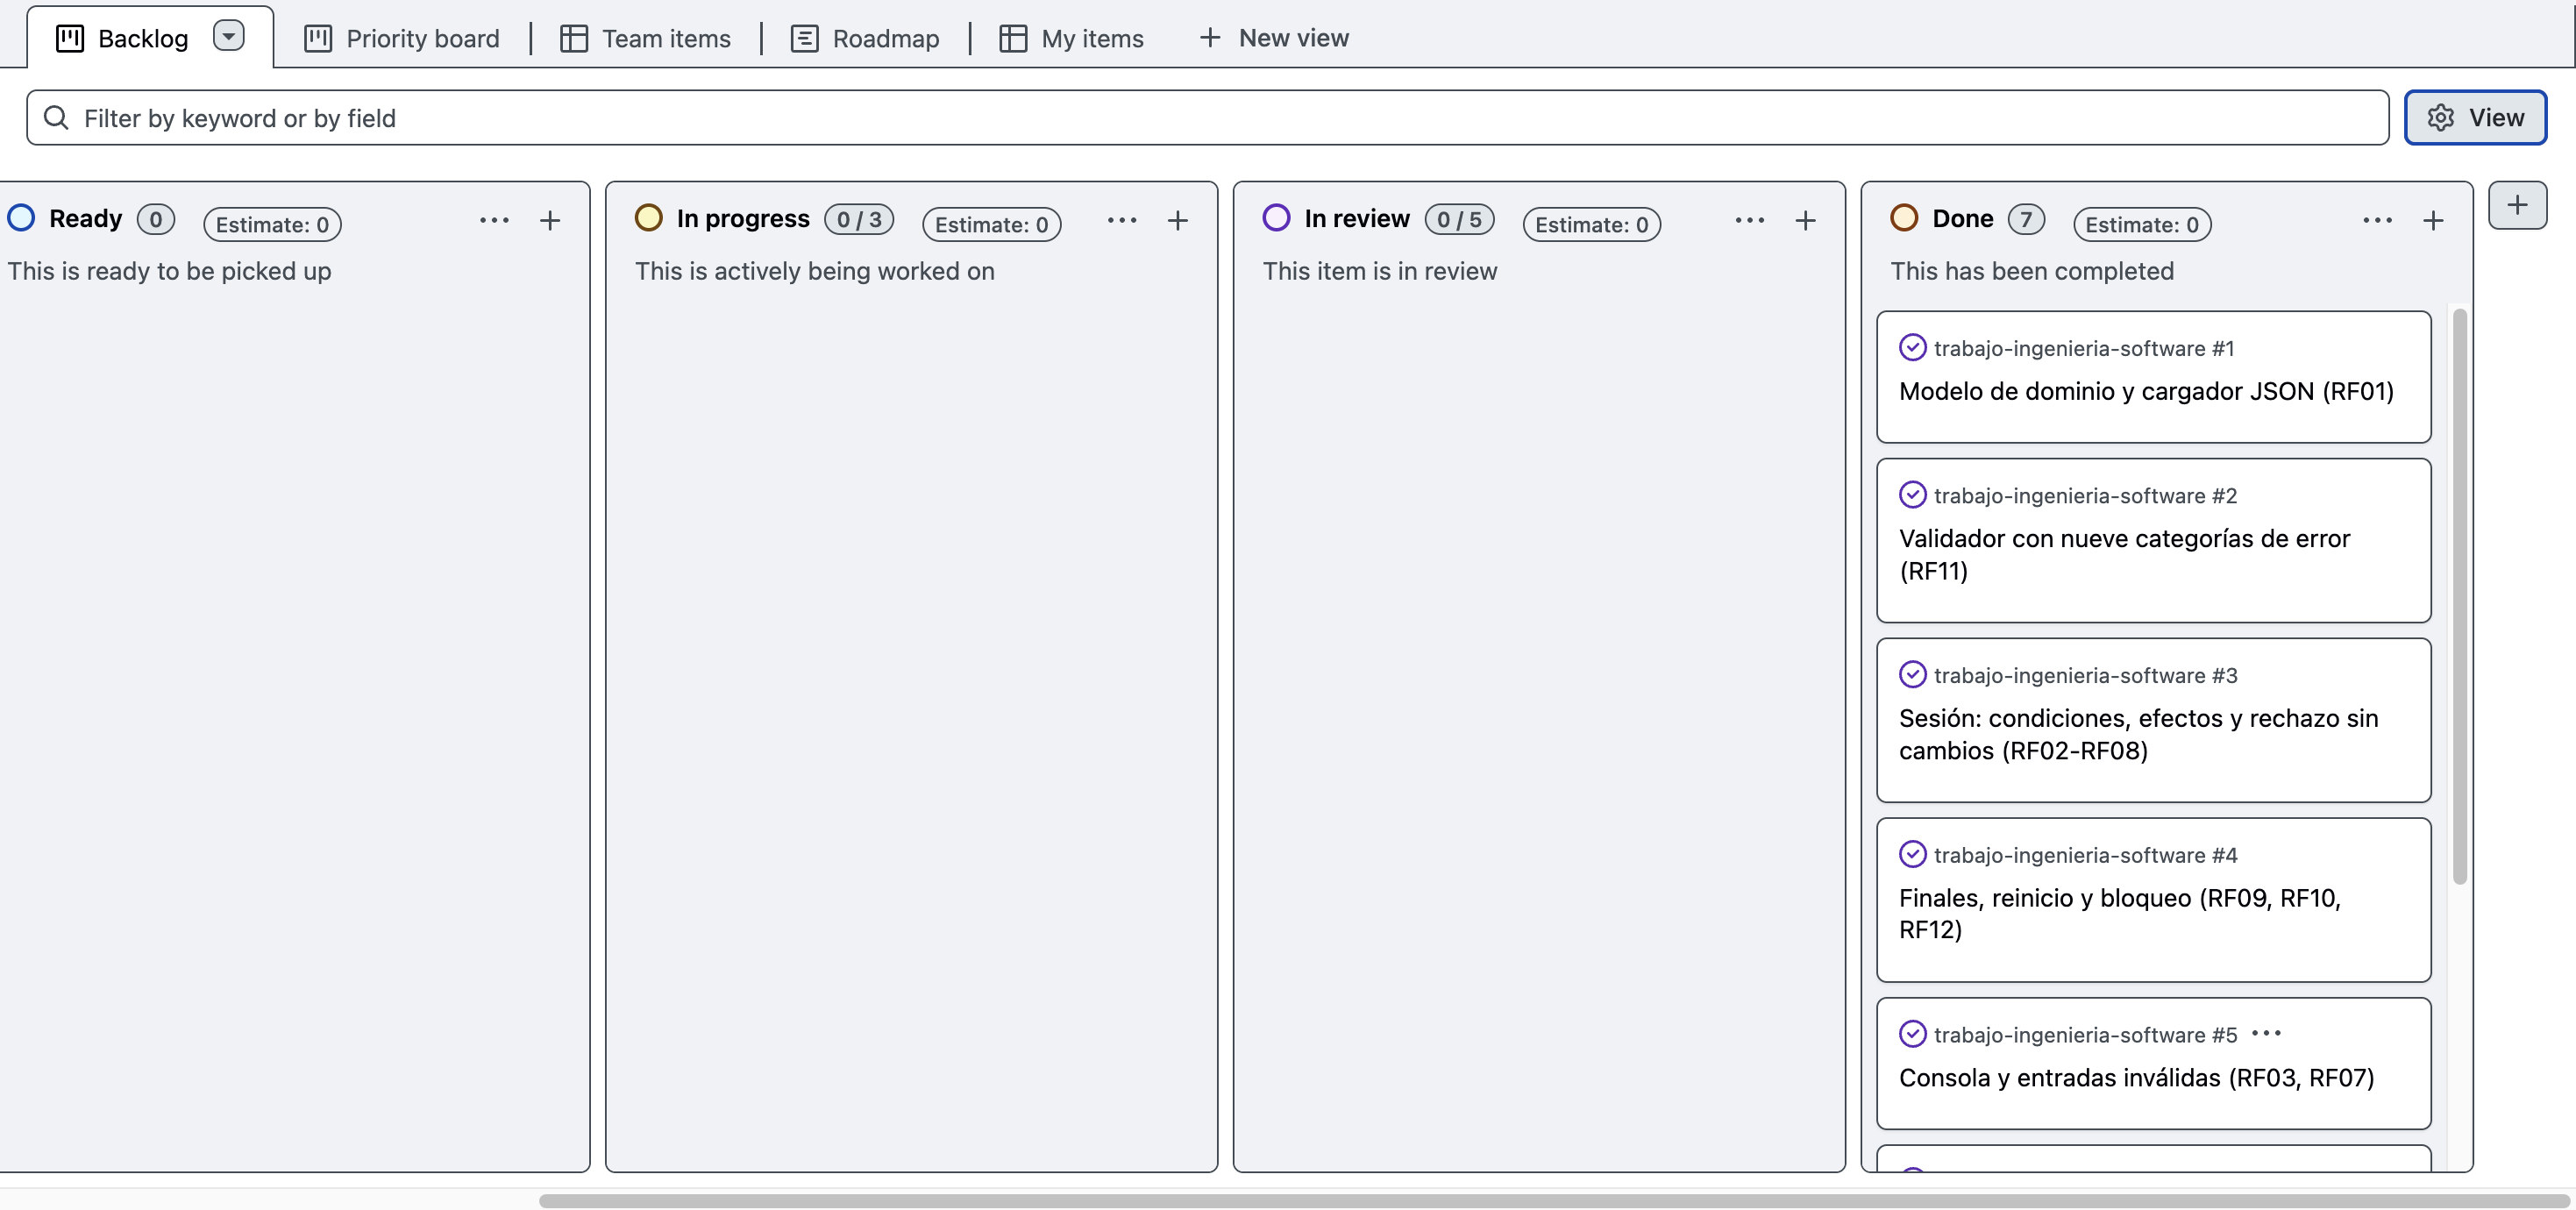
\includegraphics[width=\linewidth]{tablero_final.png}
\caption{Tablero final en GitHub Projects.}\label{fig:tablero}
\end{figure}

\end{document}
